\chapter{Cloud Computing}
\section{Definizione}
Il cloud computing è un modello che consente un accesso in rete ubiquo, agevole e su richiesta a un pool condiviso di risorse informatiche configurabili che possono essere rapidamente fornite rilasciate con il minimo sforzo di gestione o interazione con il fornitore del servizione

\section{Caratteristiche essenziali}
\begin{itemize}
    \item \textbf{Self-service su richiesta:}\\
    Gli utenti allocano le risorse automaticamente, senza alcuna interazione umana con il fornitore
    \item \textbf{Ampio accesso alla rete:}\\
    Le risorse sono accessibili attraverso la rete tramite meccanismi standard da qualsiasi dispositivo
    \item \textbf{Condivisione delle risorse:}\\
    Le risorse sono condivise tra più utenti e allocate dinamicamente in base alla richiesta
    \item \textbf{Rapida elasticità:} \\
    Le risorse scalano automaticamente e le capacità sembra illimitata all'utente
    \item \textbf{Servizio misurato:}\\
    L'utilizzo delle risorse viene automaticamente monitorato, controllato e rendicontato, garantendo trasparenza sia al fornitore che all'utente
\end{itemize}

\section{Infrastructure as a Service (IaaS)}
\begin{minipage}[c]{0.8\textwidth}
La funzionalità fornita al consumatore dal cloud provider è quella di effettuare l'allocalzione di risorse virtualizzate:
\begin{itemize}
    \item Macchine virtuali
    \item Storage
    \item Reti
    \item Atre risorse fondamentali
\end{itemize}

Il consumatore può eseguire software arbitrario sulle risorse virtualizzate senza poter però gestire e controllare la struttura del cloud
\end{minipage}
\hfill
\begin{minipage}[c]{0.2\textwidth}
    \centering
    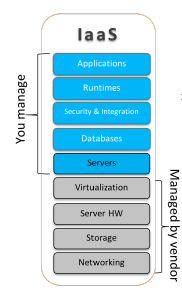
\includegraphics{figures/Schermata_20260608_162747.png}
\end{minipage}

\subsection{Architettura di sistema}
\begin{figure}[H]
    \centering
    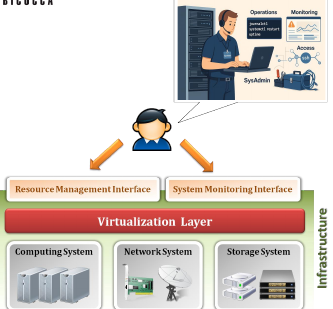
\includegraphics{figures/Schermata_20260608_163044.png}
\end{figure}
\subsubsection{RMI - Resource Monitor Interface}
Strumento che l'utente usa per creare, modificare o eliminare le proprie risorse

\subsubsection{SMI - System Monitoring Interface}
Strumento utilizzato per controllare le prestazioni, i consumi e lo stato di salute delle risorse allocate

\subsubsection{Utenti Target}
Amministratori di sistema

\section{Platform as a Service (PaaS)}
\begin{minipage}[c]{0.8\textwidth}
La funzionalità fornita al consumatore è quella di sviluppare e distribuire nel cloud applicazioni create utilizzando linguaggi di programmazione e strumenti supportati dal cloud provider.\\

Il consumatore non gestisce l'infrastruttura cloud sottostante.
\end{minipage}
\hfill
\begin{minipage}[c]{0.2\textwidth}
    \centering
    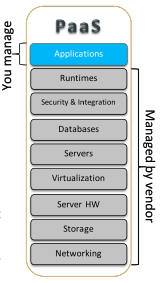
\includegraphics{figures/Schermata_20260608_163547}
\end{minipage}

\subsection{Architettura di sistema}
\begin{figure}[H]
    \centering
    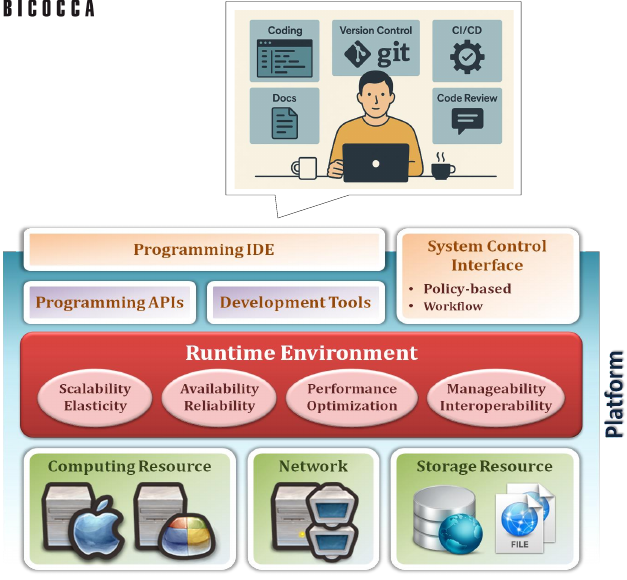
\includegraphics[scale=0.4]{figures/Schermata_20260608_164020.png}
\end{figure}
\subsubsection{Ambiente di esecuzione}
Insieme dei servizi software disponibili implementato da:
\begin{itemize}
    \item Un insieme di librerie
    \item Un motore di esecuzione delle applicazioni
\end{itemize}

\subsubsection{API di programmazione}
Utilizzata dall'utente per utilizzare i servizi messi a disposizione dall'ambiente di esecuzione

Sono differenti per cloud provider differenti, ma alcune primitive base sono comuni

\subsubsection{Interfaccia di controllo di sistema}
Punto di accesso per la gestione delle applicazioni e dell'ambiente di hosting

\section{Software as a Service (SaaS)}
\begin{minipage}[c]{0.8\textwidth}
La funzionalità fornita è quella di utilizzare le applicazioni del cloud provider eseguite su un'infrastruttura cloud \\

Il consumatore non controlla nulla dell'infrastruttura sottostante
\end{minipage}
\hfill
\begin{minipage}[c]{0.2\textwidth}
    \centering
    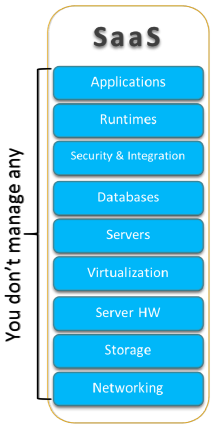
\includegraphics[scale=0.8]{figures/Schermata_20260608_164410.png}
\end{minipage}

\subsection{Architettura di sistema}
Le applicazioni web e il portale web costituiscono il thin client.

L'utente ha quindi accesso alle applicazioni eseguite remotamente in cloud.

Proprietà fondamentali portate da internet e del Web al SaaS:
\begin{itemize}
    \item \textbf{Accessibilità:}\\
    Accesso alle applicazioni ovunque
    \item \textbf{Portabilità:}\\
    Le applicazioni funzionano su qualsiasi dispositivo
\end{itemize}

\section{Cloud Pubblico}
L'infrastrttura cloud è resa disponibile al pubblico generale
\begin{itemize}
    \item Nota anche come cloud esterno o cloud multi-tenant
    \item È un ambiente cloud liberamente accessibile
    \item È proprietà di un'organizzazione che vende servizi cloud
\end{itemize}
\subsection{Caratteristiche di base}
\begin{itemize}
    \item Infrastruttura omogenea
    \item Politiche comuni
    \item Risorse condivise e multi-tenancy
    \item Infrastrutture in leasing o in affitto
    \item Economie di scala
\end{itemize}

\section{Cloud Privato}
L'infrastruttura cloud è dedicata esclusivamente a una singola organizzazione
\begin{itemize}
    \item Denominata anche cloud interno
    \item Viene limitato intenzionalmente l'accesso alle risorse ai soli utilizzatori che appartengono all'organizzazione proprietaria
    \item Può essere gestita e operata dalla stessa organizzazione o da una terza parte
    \item Può risiedere on-premise oppure off-premise
\end{itemize}

\subsection{Caratteristiche di base}
\begin{itemize}
    \item Infrastruttura eterogenea
    \item Politiche di gestione personalizzate e su misura
    \item Risorse dedicate
    \item Infrastrutture in-hosue
    \item Controllo completo
\end{itemize}

\section{Cloud di Comunità}
L'infrastruttura cloud è condivisa da diverse organizzazione
\begin{itemize}
    \item Supporta una comunità specifica che interessi e requisiti comuni
    \item L'accesso a un ambiente cloud di comunità è tipicamente limitato ai soli membri della comunità stessa
\end{itemize}

\section{Container}
\subsection{Cosa sono?}
Racchiude un'applicazione insieme a tutto ciò di cui ha bisogno per funzionare in modo che giri allo stesso modo su qualsiasi macchina

\subsection{Caratteristiche principali}
\begin{itemize}
    \item Isola l'applicazione
    \item È leggero, i container condividono lo stesso kernel del sistema operativo
\end{itemize}

\subsection{Immagini}
I container vengono creati a partire da Immagini

\subsubsection{Immagine}
\begin{itemize}
    \item Template in sola lettura utilizzato per creare i container
    \item Solitamente immagazzinata in un registro
    \item Le immagini possono essere create a partire da altre immagini
\end{itemize}

\subsubsection{Container}
\begin{itemize}
    \item Applicazione in esecuzione isolata ed effimera
    \item Autocontenuto
    \item Basato su e collegato a un'immagine specifica
\end{itemize}

\section{Container as a Service}
Modello di servizio cloud che consente agli utenti di creare e gestire container senza dover gestire l'infrastruttura sottostante

\subsection{Divisione delle responsabilità}
\begin{itemize}
    \item Il \textbf{cloud provider} gestisce l'esecuzione a runtime dei container, la rete e lo storage
    \item L'utente si concentra sullo sviluppo e sul deplou delle applicazioni containerizzate
\end{itemize}

\subsection{Vantaggi principali}
\begin{itemize}
    \item \textbf{Portabilità:}\\
    I container vengono eseguiti in modo coerente su qualsiasi provider CaaS
    \item \textbf{Scalabilità:}\\
    È possibile far scalare automaticamente i container sulla base del carico computazionale reale
    \item \textbf{Efficienza:}\\
    La natura leggera dei container riduce drasticamente l'overhead rispetto alla macchina virtuali
    \item \textbf{Ottimizzazione dei costi:}\\
    Adozione di un modello \texttt{<<pay-per-use>>} con un'allocazione delle risorse estremamente granulare
\end{itemize}

\section{I limiti del Cloud Computing}
Il modello cloud è centralizzato, questo implica sfide significative a causa della crescita esponenziale dei dispositivi IoT e dei requisiti di alcune specifiche applicazioni 

\subsection{Problematiche principali}
\begin{itemize}
    \item \textbf{Latenza:}\\
    Distanza tra i dispositivi e i datacenter crea ritardi inaccettabili per le applicazioni real-time
    \item \textbf{Larghezza di banda:}\\
    Trasmettere enormi volumi di dati grezzi dai sensori è costoso e inefficiente
    \item \textbf{Privacy:}\\
    L'invio di dati sensibili a un cloud di terze parti solleva problemi di sovranità
\end{itemize}

\section{Edge Computing}
È un paradigma di computazione distribuito che sposta la potenza di calcolo fisicamente più vicina a dove i dati vengono generati

L'edge computing consente:
\begin{itemize}
    \item Un'elaborazione dei dati più rapida
    \item Un utilizzo ridotto della larghezza di banda
    \item Garanzia di sovranità dei dati
\end{itemize}

\subsection{Modello a tre livelli}
Può essere adottato in un architettura federata che estende i servizi cloud fino ai bordi della rete e che si compone di 3 livelli:
\begin{itemize}
    \item \textbf{Livello dei terminali:}\\
    Costituito da dispositivi connessi che raccolgono dati grezzi e li inviano al livello superiore
    \item \textbf{Livello edge:}\\
    Composto da nodi edge (piccoli server) che raccolgono memorizzato ed elaborano i dati caricati dispositivi, inviando quindi i dati elaborati al cloud
    \item \textbf{Livello cloud:}\\
    Costituito da server ad alte prestazioni e dispositivi di archiviazione, dotati di potenti capacità di calcolo e di memorizzazione
\end{itemize}

\section{Fog Computing}
paradigma di computazione distribuito che fornisce risorse di calcolo e archiviazione a molteplici livelli nella gerarchia di rete.

Mentre l'edge computing si focalizza sui bordi della rete, il fog computing abilita una gerarchia fluita dall'edge al cloud

Il fog computing e l'dege computing sono complementari, il fog fornisce i carichi di lavoro che i nodi edge sono in grado di gestire